\documentclass{article}

\usepackage{times}
\usepackage{geometry}
\geometry{a4paper,left=0.6cm,right=0.7cm,top=1.5cm,bottom=1cm,columnsep=0.8cm}

\usepackage{fontawesome}          % icônes de base seulement
\usepackage[hidelinks]{hyperref}
\usepackage{multicol}
\usepackage{tikz}
\usepackage{hyphsubst}
\usepackage{moresize}
\usepackage{hyphenat}
\usepackage{tabularx}
\usepackage{ragged2e}
\usepackage{xcolor}
\usepackage{enumitem}
\usetikzlibrary{calc, positioning}
\newcolumntype{Y}{>{\RaggedRight\arraybackslash}X}

% icônes manquantes -> puce
\makeatletter
\@for\sym:=faBrain,faMicrochip,faHandshakeO,faTools,faNetworkWired,%
             faDatabase,faServer,faGit,faUsers,faComments,faCalendar,faGroup\do{%
  \@ifundefined{\sym}{\expandafter\newcommand\csname\sym\endcsname{\textbullet}}{}}
\makeatother

% couleurs
\definecolor{maincolor}{HTML}{f0fafc}
\definecolor{seccolor}{HTML}{ffffff}
\definecolor{gray}{HTML}{8c94a9}
\definecolor{sidetext}{HTML}{59cee5}

% bande latérale bleue
\usepackage{eso-pic}
\AddToShipoutPictureBG{%
  \begin{tikzpicture}[remember picture,overlay]
    \fill[maincolor] (current page.north west) rectangle
                     ([xshift=0.3\paperwidth] current page.south west);
  \end{tikzpicture}%
}

% listes
\setlist[itemize]{itemsep=-2pt,topsep=0pt,leftmargin=1.08cm}
\renewcommand{\labelitemi}{\textcolor{sidetext}{\footnotesize$\bullet$}}

\setlength{\parindent}{0pt}
\usepackage{paracol}
\columnratio{0.3}

\begin{document}
\pagestyle{empty}

\begin{paracol}{2}
% ────────────────────────────────────────
% Colonne gauche
% ────────────────────────────────────────
\color{sidetext}
\vspace*{-0.5cm}

\noindent
\begin{minipage}{\linewidth}
  \centering
  \begin{tikzpicture}
    \clip (0,0) circle (1.5cm) node[anchor=center]
      {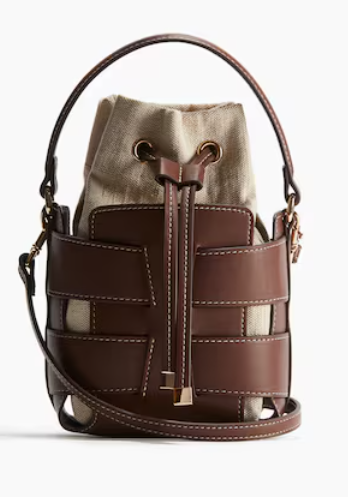
\includegraphics[width=3cm]{b0b15963e37b4e0d982b4edbe12e681d.png}};
  \end{tikzpicture}

  \vspace{3mm}
  {\color{black}\LARGE \textbf{Judikael Mourouvin}}

  \vspace{1mm}
  {\large Alternant en Marketing Digital}

  \vspace{3mm}
  {\color{gray}\rule{\linewidth}{0.4pt}} \\
\end{minipage}

% ── Coordonnées
\begin{tabular}{@{}c l}
  \faPhone &
  \begin{tabular}[t]{@{}l@{}}
    {\color{gray}Téléphone} \\ +590 0690 91 14 48
  \end{tabular} \\
  \\
  \faLinkedin &
  \begin{tabular}[t]{@{}l@{}}
    {\color{gray}LinkedIn} \\
    \href{}{Mon LinkedIn}
  \end{tabular} \\
  \\
  \faMapMarker &
  \begin{tabular}[t]{@{}l@{}}
    {\color{gray}Adresse} \\ Route de COCOYER \\ 97190 GOSIER
  \end{tabular} \\
  \\
  \faEnvelope &
  \begin{tabular}[t]{@{}l@{}}
    {\color{gray}Email} \\
    \href{mailto:jkmou971@gmail.com}{jkmou971@gmail.com}
  \end{tabular} \\
\end{tabular}

\vspace{2mm}
{\color{gray}\rule{\linewidth}{0.4pt}} \\

% ── Langues --------------------------------------------------------
{\color{black}{Langues}}

\vspace{2mm}
\begin{itemize}[leftmargin=*]
\item English - \textcolor{gray}{}
\item Espagnol - \textcolor{gray}{}\end{itemize}          % ← le placeholder va contenir \begin{itemize}…\end{itemize}

{\color{gray}\rule{\linewidth}{0.4pt}} \\

% ── Compétences ----------------------------------------------------
\vspace{2mm}
{\color{black}{Compétences Clés}}

\vspace{2mm}
\begin{itemize}[leftmargin=*]
\item Administration
\item Réseaux
\item Assistance
\item Diagnostic
\item Maintenance
\item Configuration
\item Support\end{itemize}              % ← idem, une vraie liste
\vspace{2mm}
{\color{gray}\rule{\linewidth}{0.4pt}} \\

% ── Centres d'intérêt
\vspace{2mm}
{\color{black}{Centres d’intérêt}}

\vspace{2mm}
\begin{itemize}[leftmargin=*]
\item Lectur
\item Sports
\item Musique
\item Voyage
\end{itemize}     % ← simple itemize ou tabular

\vfill
~

% ────────────────────────────────────────
\switchcolumn
% Colonne droite
% ────────────────────────────────────────
\color{black}

% ── Profil
\textcolor{black}{\Large \textbf{Profil Professionnel}} \\[2pt]
Passionné par l’informatique et le marketing digital, je possède une expérience confirmée en support technique et en gestion de projets numériques. Mon alternance à la DSI de la Mairie du Gosier m’a permis de renforcer mes compétences en administration réseaux, assistance utilisateur et stratégie digitale. Autonome et rigoureux, j’interviens aussi bien sur la maintenance des postes que sur la mise en place de solutions marketing. Je souhaite désormais mettre cette polyvalence au service de nouveaux défis à temps plein. \\[8pt]

% ── Expérience
\textcolor{black}{\Large \textbf{Expérience Professionnelle}} \\[2pt]

\colorbox{maincolor}{%
  \begin{minipage}{\linewidth}
    \textbf{Alternant en Marketing Digital}              2023-2024  \\ Mairie du Gosier, DSI 
    \begin{itemize}
      \item Coordonné divers projets numériques, assurant leur livraison dans les délais impartis. \item Analysé les besoins des agents et déployé des solutions digitales adaptées. \item Formé les utilisateurs et soutenu la stratégie de marketing en ligne de la collectivité.
    \end{itemize}
  \end{minipage}}

\vspace{3mm}


\colorbox{maincolor}{%
  \begin{minipage}{\linewidth}
    \textbf{Animateur de la zone informatique}              2022-2023  \\ POLE EMPLOI, Gosier 
    \begin{itemize}
      \item Fournit un support de proximité aux utilisateurs, résolvant rapidement leurs incidents. \item Configuré et entretenu les postes de travail, garantissant la disponibilité du parc. \item Diagnostiqué pannes matérielles et logicielles, réduisant les interruptions de service.
    \end{itemize}
  \end{minipage}}

\vspace{3mm}


\colorbox{maincolor}{%
  \begin{minipage}{\linewidth}
    \textbf{Stagiaire Informaticien}              2020-2021  \\ NUMERIKA, Baie Mahault 
    \begin{itemize}
      \item Configuré et maintenu le parc informatique, améliorant la performance du réseau. \item Assuré le support utilisateur quotidien, renforçant la satisfaction interne.
    \end{itemize}
  \end{minipage}}   % ← blocs \colorbox{maincolor}{\begin{minipage}…}

\vspace{8mm}

% ── Formation
\textcolor{black}{\Large \textbf{Formation}} \\[2pt]

\begin{tabularx}{\linewidth}{@{}c  >{\RaggedRight\arraybackslash}X
                             >{\raggedleft\arraybackslash}p{0.25\linewidth}@{}}
\textcolor{sidetext}{\faGraduationCap} &
\textbf{Bachelor Marketing Digital} &
\textit{2023-2024} \\
& CFA IUTS & \\   % ligne de l’établissement
\end{tabularx}
\begin{itemize}[leftmargin=*]
  \item Étudié les fondamentaux du marketing en ligne : SEO, SEA et réseaux sociaux.
  \item Réalisé des projets de stratégie digitale et d’analyse de performance.
  \item Développé des compétences en gestion de contenu et outils d’automatisation.
\end{itemize}
\vspace{3mm}

\begin{tabularx}{\linewidth}{@{}c  >{\RaggedRight\arraybackslash}X
                             >{\raggedleft\arraybackslash}p{0.25\linewidth}@{}}
\textcolor{sidetext}{\faGraduationCap} &
\textbf{BTS Système Numérique option Informatique et Réseaux} &
\textit{2019-2021} \\
& Lycée de Chevalier Saint Georges, Abymes & \\   % ligne de l’établissement
\end{tabularx}
\begin{itemize}[leftmargin=*]
  \item Approfondissement de l’architecture réseau et de la configuration d’équipements actifs.
  \item Pratique de la maintenance matérielle et logicielle de systèmes informatiques.
  \item Acquisition de bases solides en programmation et cybersécurité.
\end{itemize}       % ← lignes tabular par diplôme

\end{paracol}
\end{document}

